\documentclass[a4paper, top=10mm]{article}
%for writing from the top
\usepackage{fullpage}
%for math
\usepackage{amsmath}
\usepackage{mathrsfs}
\usepackage{amsthm}
%for images
\usepackage{graphicx}
%for color
\usepackage{xcolor}
%for title
\title{\textbf{\huge{Chasse a l'angle}}}
\author{Enigma n\textsuperscript{o}3}
\date{16\textsuperscript{th} June 2026}

\newtheorem*{hint}{Hint}

\addtolength{\voffset}{-2cm}
\addtolength{\textheight}{5cm}


\begin{document}
	\maketitle
	
	\Large
	
	Soient $A$, $B$, $C$ alignes tel que $[AB] = 2 \times [BC]$.
	Soit $D$ tel que $\angle ABD$ vaut 60 degres, et $\angle ACD$ vaut 45 degres.
	
	Combien vaut $\angle BAD$?
	
	
	\vspace{3cm}
	
	Let $A$, $B$, and $C$ be collinear such that $[AB] = 2 \times [BC]$.
	Let $D$ be such that $\angle ABD$ is 60 degrees, and $\angle ACD$ is 45 degrees.
	
	What is the value of $\angle BAD$?
	
	\vspace{3cm}
	
	\begin{center}
		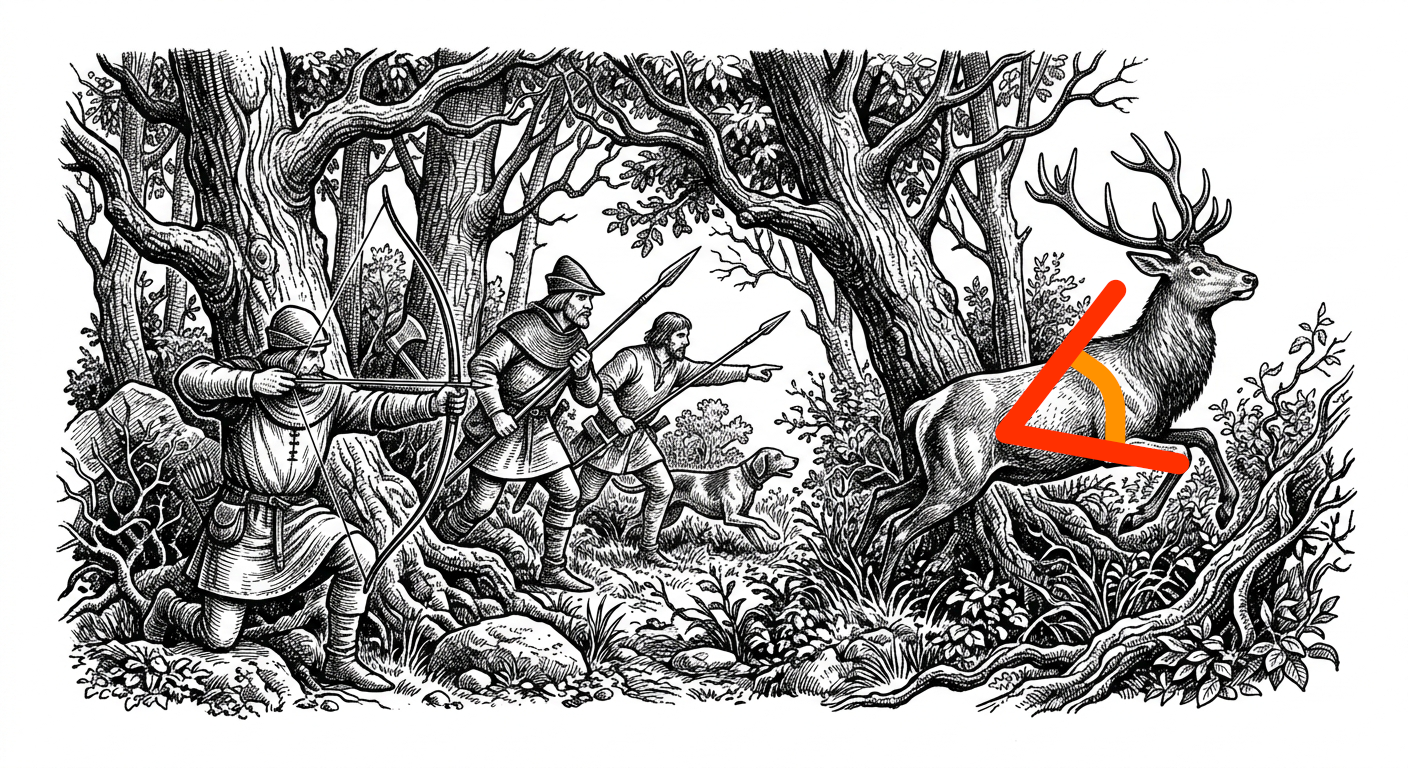
\includegraphics[width=\linewidth]{03angle_hunt.png}
	\end{center}
	
	% \angle BAD = 75 degree
	
	
\end{document}